%!TEX root = ../../PhD_thesis__Edouard_Leurent.tex

\graphicspath{{2-Chapters/2-Chapter/}}

\chapter{Literature Review}
\label{chapter:2}

\begin{flushright}
	\begin{tabular}{@{}l@{}}
		\emph{Souhaite que la route soit longue. [\dots]}\\
		\emph{Visite aussi beaucoup de villes égyptiennes,}\\
		\emph{et n’aie de cesse de t’instruire auprès de ceux qui savent.}\\
	\end{tabular}
	
	Konstantinos Kavafis, \href{https://eleurent.github.io/sisyphe/texts/ithaki.html}{\emph{Ithaque}}.
\end{flushright}

\section{Sequential decision-making}
\label{sec:sequential-decision-making}

The skill of driving a car involves taking a series of decisions, where early stages influence the resulting outcomes and subsequent reasoning at late stages. This aspect is known as sequential (or multistage) decision-making. Let us start by introducing some useful notations. At each time step $t$, the system is described by its \emph{state} $s_t$ that belongs to a measurable state space $\cS$. Then, the agent can take an \emph{action} $a_t$ within a measurable action space $\cA$, before transitioning to a next state $s_{t+1}\in\cS$, drawn from a conditional distribution $P\parentheses{s_{t+1} \mid s_t, a_t}$ that we call the \emph{system dynamics}. The agent actions can themselves be drawn from a distribution $\pi\parentheses{a_t\mid s_t}$, called the \emph{policy}. This section describes the main design principles for coming up with a good driving policy $\pi$.

\subsection{Motion Planning}

The development of motion planning techniques for intelligent vehicles date back to the late 80s, supported by international research projects such as Eureka (1987) of the Prometheus program, followed by the DARPA Grand and Urban Challenges (2004, 2007), and more recently the VIAC (2010), GCDC (2011) and Delphi (2015) challenges. In two surveys \citep{Gonzalez2016,Paden2016} studying the literature of this period, three main approaches have been identified.

\paragraph{Search-based algorithms}

This method is based on a regular discrete partition of the state space $\cS$ called a \emph{lattice}, which must be connected by feasible trajectories \citep[\eg][]{Pivtoraiko2005}. This framing reduces motion planning to the problem of finding a shortest path in a known graph. Then, traditional graph-search algorithms such as Dijkstra's algorithm \citep{Dijkstra1959}, $A^\star$ \citep{Hart1968} or $D^\star$ \citep{Stentz1994} can been used to compute the optimal trajectory. This technique has been applied by at least five different teams during the DARPA Urban Challenge for driving on structured roads and unstructured parking: Dijkstra for team Ben Franklin \citep{Bohren2008} and VictorTango \citep{Bacha2008}, and $A^\star$ for Stanford University \citep{Montemerlo2008} and KIT \citep{Kammel2008}, and $D^\star$ by the winning team from CMU \citep{Urmson2008}.

\begin{figure}[tp]
	\centering
	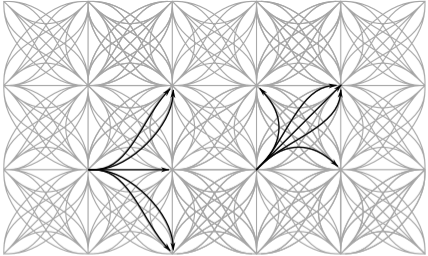
\includegraphics[width=0.5\linewidth]{img/lattice2}
	\caption{A lattice structure connects a discrete set of states by feasible trajectories}
\end{figure}

\paragraph{Sampling-based algorithms}

The limitation of search-based algorithms lies in the difficulty of formulating a regular lattice structure covering the states space $\cS$ with feasible transitions, and in the real-time constraint that may not be met by graph-search algorithms. To address them, sampling-based motion planners iteratively grow a set of reachable configurations by randomly sampling valid transitions. The most popular ones are Probabilistic Roadmap (PRM) \citep{Kavraki1996}, Rapidly-exploring Random Trees (RRT) \citep{Lavalle98,Karaman2011} and Monte-Carlo Tree Search algorithms \citep[e.g.][]{Kocsis2006}.
\TODO{these methods have been used in the context of AD in...}

\paragraph{Optimisation-based algorithms}

The third approach consists in optimizing a parametrized trajectory with respect to a real-valued objective function. The most popular instance is interpolation between the current and goal states, which has been applied to various classes of functions in the context of Autonomous Driving, such as lines and circles \citep{Reeds1990}, clothoids \citep{Funke2012}, polynomials \citep{Xu2012}, and Bézier curves \citep{Gonzalez2016}.

Motion planning techniques thus rely on deterministic models of the vehicle dynamics. These models are often required to take a simple form so that the search or optimisation procedure can be solved efficiently, which prevents from considering couplings and interactions with other vehicles. Therefore, other objects are most often considered static, or with simplistic behaviours. 

\paragraph{Collaborative planning}

The difficulty of predicting complex interactions patterns in the multi-agent setting can be bypassed in one particular setting: cooperative motion planning for multiple vehicles.
\TODO{collaborative planning, centralized (joint behaviour is optimised): does not allow human drivers, uncertainty. example ref: https://ieeexplore.ieee.org/document/736775}


\subsection{Imitation Learning}

An orthogonal strategy to motion planning techniques is to learn a reactive policy $\pi(a|s)$ under supervision of an expert $\pi_E$ that produces a dataset $\cD$ of demonstration trajectories. To that end, a parametrized policy $\pi_\theta$ is optimised to minimise a regression loss $\cL$, for instance the $KL$ divergence to the expert actions distribution:
\begin{equation*}
\min_\theta \expectedvalue_{s\sim \cD} \left[\cL\left(\pi_{\theta}(a|s), \pi_E(a|s)\right)\right]
\end{equation*}
This approach is also referred to as behavioural cloning, and is particularly suited when only low-level high-dimensional inputs are available, such as camera images, which prevents access to the dynamics model required by motion planning approaches. 
The first application of imitation learning to autonomous driving is the ALVINN (Autonomous Land Vehicle In a Neural Network) project \citep{Pomerleau89}, where a 3-layer neural network was trained for the task of road following, as shown in \Cref{fig:alvinn}.
\begin{figure}[tp]
	\centering
	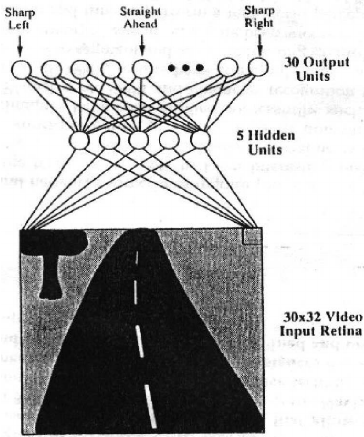
\includegraphics[width=0.4\linewidth]{img/alvinn}
	\caption{The 3-layer architecture used in ALVINN \citep{Pomerleau89}.}
	\label{fig:alvinn}
\end{figure}

\paragraph{Compounding errors} Unfortunately, the behavioural cloning paradigm is known to suffer from \emph{compounding errors}: since the future states depend on previous predictions (actions), the \iid assumption made in statistical learning does not hold. Therefore, small mistakes will place the system into states that are outside the training data distribution, as illustrated in \Cref{fig:compounding}, and resulting policies struggle to maintain high performances on long time horizons. This effect was identified and tackled in \citep{Ross2011}, who proposed to iteratively request expert labels (actions) from the states encountered by the current trained policy, rather than from the initial expert distribution. However, this can only be accomplished at the cost of a significant labelling effort. 
\begin{figure}[tp]
	\centering
	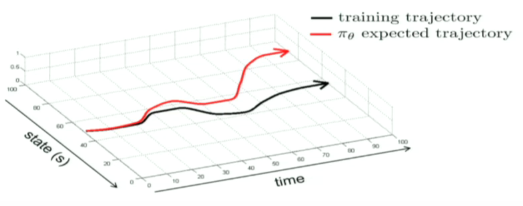
\includegraphics[width=0.7\linewidth]{img/cp4}
	\caption{As the agent deviates from the expert trajectories, the errors compound and push the agent further and further from the training distribution.}
	\label{fig:compounding}
\end{figure}
In the context of a Lane Keeping application, \citep{Bojarski2016} proposed instead to mitigate this issue during the data collection step by simulating deviations from the expert trajectories by means of two side cameras facing at the edge of the road. The corresponding synthetic expert controls were obtained by adding a constant adjustment term steer the vehicle back on track. The effect of compounding errors can also be delayed by further increasing the prediction performance, \eg by considering temporal dependencies as in \citep{Eraqi2017,Xu2017}. Other techniques than maximum likelihood estimation can be used to train the models, such as Generative Adversarial Imitation Learning \citep{Ho2016}, used for highway driving from range measurements in \citep{Kuefler2017,Bhattacharyya2018}.

\paragraph{Policy conditioning} A limitation of imitation learning for autonomous driving is fact that simply imitating human drivers by sampling likely trajectories is not sufficient: the sampling must also be conditioned on the current short-term destination specified by the Route planner. \citep{Codevilla2018} propose to achieve this by considering several policy heads for three possible behaviours when reaching an intersection: go straight, turn left or turn right. At test time, the appropriate policy is used at each intersection depending on the planned route. \citep{Rhinehart2020} present a more general approach that consists in learning a probabilistic model $q(s)$ of expert trajectories used as a prior, and inferring the maximum a posteriori trajectory given a test-time goal likelihood $p\parentheses{goal\mid s}$.

\subsection{Reinforcement Learning}

Reinforcement Learning is a general framework for learning-based sequential decision-making. It is formulated as an optimal control problem: the policy $\pi$ is chosen to optimise an objective function. It is generally formalized as a \emph{Markov Decision Process} (MDP), a tuple $(\cS, \cA, P, R, \Gamma)$ in which at each step, a bounded reward $r_t\in[0, 1]$ drawn from a reward distribution $R(r_t|s_t,a_t)$. The agent must act so as to optimise in expectation its cumulative discounted reward, also called \emph{return}, where $\gamma\in[0,1)$ is the discount factor:

\begin{equation*}
\max_{\pi}\expectedvalue_{\pi, P} \left[\sum_t \gamma^t r_t\right].
\end{equation*}

\TODO{Several performance measures: return, cumulative regret, simple regret, PAC}

Convenient framework for analysis, but it's often too narrow a frame for the real world to fit in. In the following, we will enumerate several assumptions behind the MDP framework that may not hold in practice, and for which variants have been developed. We will focus on applications of the variants the particular context of Autonomous Driving.

\section{States and partial observability}

\begin{figure}[tp]
	\centering
	\begin{subfigure}[b]{.7\linewidth}
		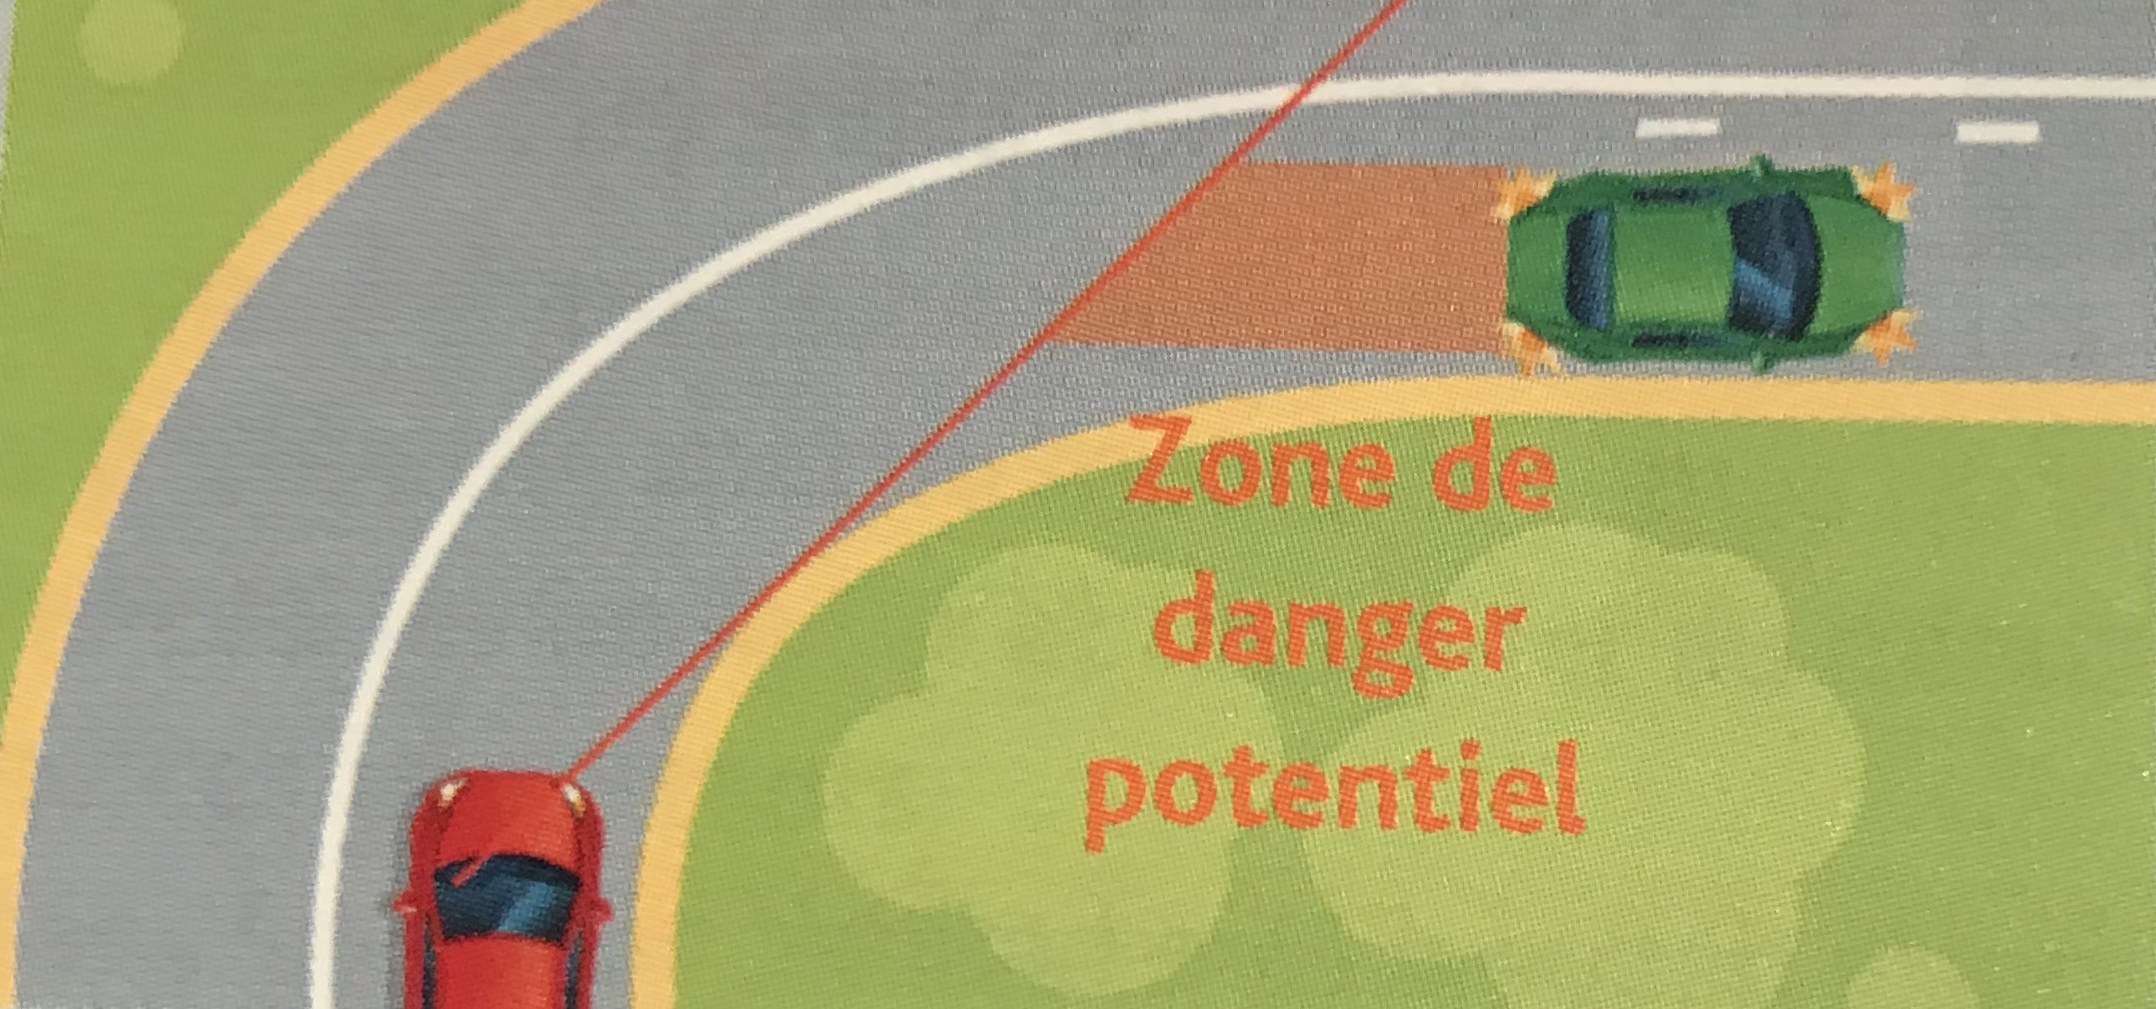
\includegraphics[width=\linewidth]{img/po-sensors}
		\caption{"Area of potential danger". A partial observability stemming from sensor occlusion in a turn.}
		\label{fig:po-occlusion}
	\end{subfigure}
	\begin{subfigure}[b]{.4\linewidth}
		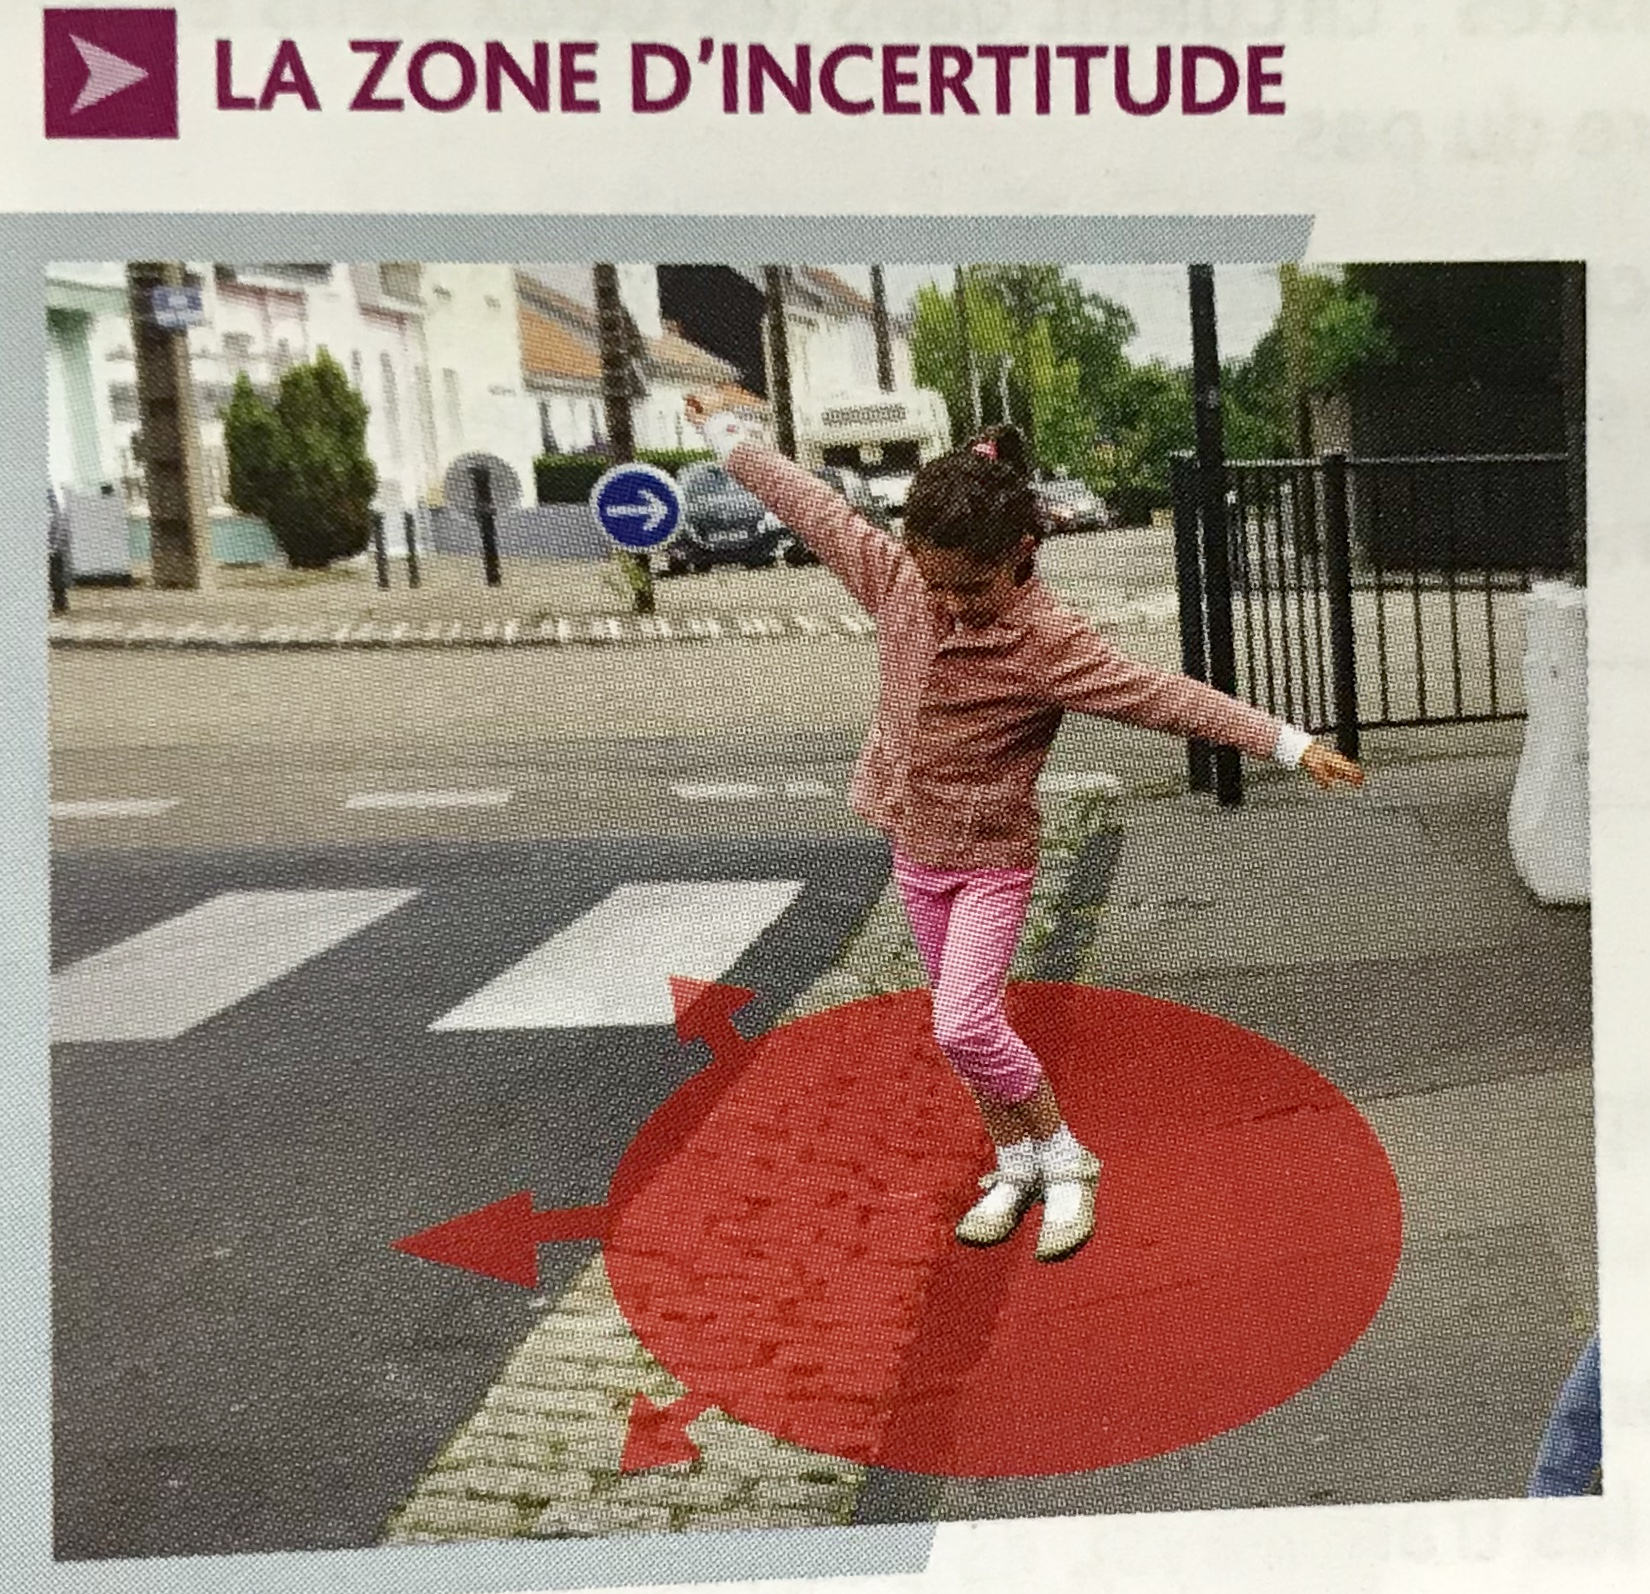
\includegraphics[width=\linewidth]{img/po-intentions}
		\caption{"Area of uncertainty". A partial observability stemming from unknown intentions of human agents.}
		\label{fig:po-intentions}
	\end{subfigure}
	\caption{Sources of Partial Observability in Autonomous Driving. Illustrations from \citep{ObjCode2017}.}
	\label{fig:partial-observability}
\end{figure}
\begin{figure}
	\centering
	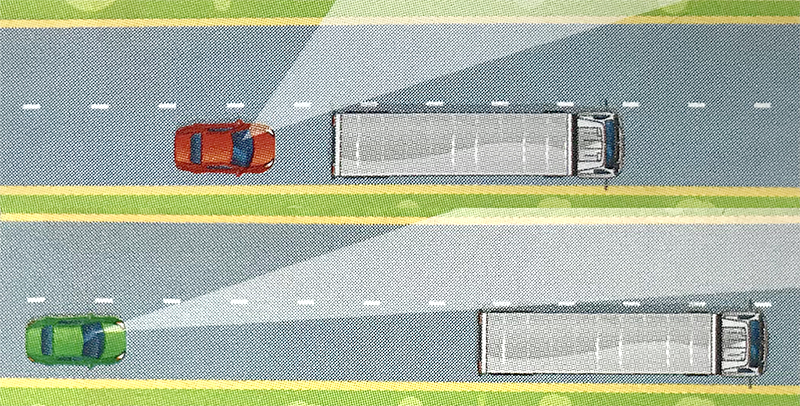
\includegraphics[width=0.7\linewidth]{img/pomdp}
	\caption{Information-seeking behaviours: the tailgating vehicle (top) should slow down, although it might decrease its immediate rewards, to gain valuable information in return (bottom). Image from \citep{ObjCode2017}.}
	\label{fig:information-seeking}
\end{figure}

The MDP framework is based on the hypothesis that the agent has access to its own state $s\in\cS$. In practice, information about the scene can only be obtained through sensors, which produce typically noisy measurements \citep{Ulbrich2013,Du2010}. Worse, parts of the state may be missing altogether, as is the case when a scene entity is occluded by an obstacle \citep[\eg][]{Brechtel2013,Bouton2018,Sun2019}, as shown in \Cref{fig:po-occlusion}. To account for these difficulties, the concept of a \emph{Partially Observable} Markov Decision Process (POMDP) was introduced in \citep{Astrom1965}, extending the MDP framework with two additional quantities: an observation space $\Omega$, and an measurement model $O$ such that the observation $o\in\Omega$ is measured at state $s'$ with the conditional probability $O\parentheses{o\mid s',a}$. At each time step $t$, a belief $b_t\in\cM(\cS)$ over the state $s_t\in \cS$ is updated by performing Bayesian Filtering to compute the posterior state distribution:
\begin{equation*}
b_{t+1}(s_{t+1}) = \frac{O(o_t|s_{t+1}, a_t)\sum_{s_{t}\in\cS}P\parentheses{s_{t+1} \mid s_t, a_t}b_t(s_t)}{\sum_{s\in\cS} O(o_t|s, a_t)\sum_{s_{t}\in\cS}P\parentheses{s \mid s_t, a_t}b_t(s_t)}.
\end{equation*}
By conditioning the policy $\pi(a_t|b_t)$ on the belief $b_t$, the POMDP framework allows to optimally balance between information gathering and task completion, as shown in \Cref{fig:information-seeking}. However, there is a price to pay: the belief space $\cM(\cS)$ is much larger than the state space $\cS$ (\eg continuous of dimension $n$ when $\cS$ is finite of size $n$), which drastically increases the planning complexity. Exact solutions exist when $\cS$ is finite \citep{Pineau2003}, and approximate ones when it is compact \citep{Porta2006,Silver2010}. Even the belief update is intractable in general, when $\cS$ is compact. In the case of linear dynamics and Gaussian measurement noise, the belief update is known as Kalman Filtering \citep{Kalman1960}. It has been applied in \citep[\eg]{Bry2011,Bouton2017,VanDenBerg2017}, and in the context of quadratic costs --\ie the standard LQG problem-- which enables efficient computation of the optimal policy \citep[see e.g.][]{Xu2014,VanDenBerg2011}. The more complex observation model of sensor occlusions in continuous-space is handled in \citep{Brechtel2013,Brechtel2014,Bouton2018} where cautious driving policies are learned for crossing intersections; and in \citep[][]{Sun2019} where the observed behaviour of nearby vehicles is used to infer the presence of potentially occluded pedestrians.
Furthermore, the POMDP framework has been used to account for uncertainty in the intentions of other agents, as illustrated in \Cref{fig:po-intentions}. In \citep{Bandyopadhyay2013}, the authors propose a Mixed-Observability framework (MOMDP) in which the other drivers locations are observed but not their destinations. In \citep{Barbier2018}, the uncertainty lies in whether the other agents intend to yield of take the right of way.

- \citep{Sunberg2017}: evaluate the POMDP vs MDP approximation with an assumed internal state.

- \citep{VanDenBerg2017}


\section{Actions and temporal abstraction}

Driving involves reasoning at several time scales: which route to take in the next minutes? how to coordinate with other agents in the next dozen of seconds? what throttle and steering controls to apply in the next second?
Temporal abstraction: the notion of low-level actions and high-level temporally extended skills called \emph{options}. Hierarchical reinforcement learning.

The semi-Markov framework
Plan with options: temporally-extended sequences of actions
Hierarchical structure: learn skills that can be reused as actions

When humans lean to drive, control of the steering wheel and throttle/brake pedals is acquired in a few hours. 
Instructor: Deciding when to change lane, overtake, give or take way, proceed at an intersection, etc.
Semantic action space

In autonomous driving, this hierarchy is typically imposed by the robotics pipeline presented in \Cref{chapter:1}. 
Can also be learned: Option graph on the double merge scenario: [Safe, Multi-Agent, Reinforcement Learning for Autonomous Driving]
Learned locomotion skills (follow, overtake) used as meta-actions: [Combining Neural Networks and Tree Search for Task and Motion Planning in Challenging Environments, ]

Shorter action duration means smaller signal-to-noise ratio, which leads to slow learning [“On a Formal Model of Safe and Scalable Self-driving Cars]

\citep{Barbier2018}: Stop, yield, pass

\section{Rewards and inverse reinforcement learning}


\citep{Sun2019}: estimate driver preferences
\citep{Sadigh2016}: model the human as an optimal planner, reward learnt with IRL.

\section{Dynamics and transfer}
\section{Optimisation criterion and safety}
